\subsubsection{UC\theuccount-CE - Gestore Personale invia il messaggio finale al Consumer Email}
%	\begin{figure}[H]
%		\centering
%		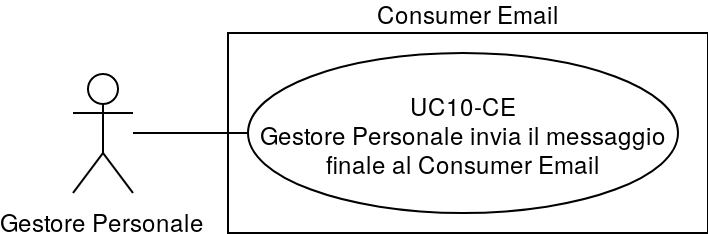
\includegraphics[width=0.6\textwidth]{img/casi_d'uso/UC10.png}\\
%		\caption{UC\theuccount-CE - Gestore Personale invia il messaggio finale al Consumer Email}
%	\end{figure}
	\begin{itemize}
		\item \textbf{Codice}: UC\theuccount-CE.
		\item \textbf{Titolo}: Gestore Personale invia il messaggio finale al Consumer Email.
		\item \textbf{Attori primari}: Gestore Personale.
		\item \textbf{Descrizione}: il Gestore Personale, dopo aver ricevuto il messaggio elaborato
		dal Producer Redmine o GitLab, controlla i Topic del messaggio, gli utenti iscritti, la loro disponibilità e se la loro preferenza è Email.
		Se tutte queste condizioni sono verificate, viene preparato il messaggio finale da inviare successivamente viene inviato al Consumer Email. 
		Se il destinatario è iscritto a quel Topic ma non è disponibile, il destinatario viene cambiato con la persona di fiducia. \par
		Il messaggio finale, una volta elaborato, conterrà i campi:
		\begin{itemize}
			\item Email del destinatario
			\item Applicazione di provenienza
			\item Ora di invio
			\item Tipo di segnalazione(commit, issue)
			\item Project
			\item Topic
			\item Subject e opzionalmente
		 	\begin{itemize}
				\item Description
				\item Due date
				\item Milestone
				\item Assignee
			\end{itemize}
		\end{itemize}
		\item \textbf{Precondizione}: il Gestore Personale ha ricevuto il messaggio elaborato dal Producer Redmine o GitLab.
		\item \textbf{Postcondizione}: Il Gestore Personale ha inviato il messaggio finale al Consumer Email.
		\item \textbf{Scenario principale}: 
		\begin{enumerate}
			\item ll Gestore Personale riceve un messaggio dal Producer Redmine o dal Producer GitLab
			\item Il Gestore Personale valuta quali utenti sono iscritti al Topic del messaggio ricevuto e se vogliono ricevere il messaggio tramite Email
			\item Il Gestore Personale procede all'invio del messaggio finale al Consumer Email
		\end{enumerate}
		
	\end{itemize}